\section{Appendix}

% Table created by stargazer v.5.2.2 by Marek Hlavac, Harvard University. E-mail: hlavac at fas.harvard.edu
% Date and time: Sun, Apr 02, 2023 - 12:08:09 PM
\begin{table}[!htbp] \centering 
  \caption{Larger extract of vanilla regression table} 
  \label{appendix Larger extract of vanilla regression table} 
\begin{tabular}{@{\extracolsep{5pt}}lc} 
\\[-1.8ex]\hline 
\hline \\[-1.8ex] 
 & \multicolumn{1}{c}{\textit{Dependent variable:}} \\ 
\cline{2-2} 
\\[-1.8ex] & slum \\ 
\hline \\[-1.8ex] 
  Light Bin 4 and Pop Density Bin 0 & 2.611$^{***}$ \\ 
  & (0.404) \\ 
  & \\ 
 Light Bin 0 and Pop Density Bin 1 & 1.988$^{***}$ \\ 
  & (0.398) \\ 
  & \\ 
 Light Bin 0 and Pop Density Bin 2 & 1.851$^{***}$ \\ 
  & (0.397) \\ 
  & \\ 
 Light Bin 0 and Pop Density Bin 3 & 1.928$^{***}$ \\ 
  & (0.397) \\ 
  & \\ 
 Light Bin 0 and Pop Density Bin 4 & 1.430$^{***}$ \\ 
  & (0.398) \\ 
  & \\ 
 Light Bin 4 and Pop Density Bin 1 & $-$2.050$^{***}$ \\ 
  & (0.410) \\ 
  & \\
 Light Bin 4 and Pop Density Bin 2 & $-$1.802$^{***}$ \\ 
  & (0.409) \\ 
  & \\ 
 Light Bin 2 and Pop Density Bin 3 & 0.903$^{*}$ \\ 
  & (0.540) \\ 
  & \\
 Light Bin 4 and Pop Density Bin 3 & $-$1.417$^{***}$ \\ 
  & (0.409) \\ 
  & \\ 
 Light Bin 3 and Pop Density Bin 4 & $-$0.765$^{*}$ \\ 
  & (0.453) \\ 
  & \\ 
 Light Bin 4 and Pop Density Bin 4 & $-$2.085$^{***}$ \\ 
  & (0.409) \\ 
  & \\ 
\hline \\[-1.8ex] 
Observations & 31,810 \\ 
Log Likelihood & $-$20,911.600 \\ 
Akaike Inf. Crit. & 41,863.200 \\ 
\hline 
\hline \\[-1.8ex] 
\textit{Note:}  & \multicolumn{1}{r}{$^{*}$p$<$0.1; $^{**}$p$<$0.05; $^{***}$p$<$0.01} \\ 
\end{tabular} 
\end{table} 

% Table created by stargazer v.5.2.2 by Marek Hlavac, Harvard University. E-mail: hlavac at fas.harvard.edu
% Date and time: Sun, Apr 02, 2023 - 12:11:57 PM
\begin{table}[!htbp] \centering 
  \caption{Larger extract of bins regression table} 
  \label{appendix Bins Regression Table} 
\begin{tabular}{@{\extracolsep{5pt}}lc} 
\\[-1.8ex]\hline 
\hline \\[-1.8ex] 
 & \multicolumn{1}{c}{\textit{Dependent variable:}} \\ 
\cline{2-2} 
\\[-1.8ex] & slum \\ 
\hline \\[-1.8ex] 
Light Bin 0 and Pop Density Bin 8 & 1.632$^{***}$ \\ 
  & (0.400) \\ 
  & \\ 
 Light Bin 0 and Pop Density Bin 9 & 0.898$^{**}$ \\ 
  & (0.406) \\ 
  & \\ 
 Light Bin 8 and Pop Density Bin 1 & $-$0.998$^{**}$ \\ 
  & (0.453) \\ 
  & \\ 
 Light Bin 9 and Pop Density Bin 1 & $-$1.562$^{***}$ \\ 
  & (0.467) \\ 
  & \\ 
 Light Bin 8 and Pop Density Bin 2 & $-$1.458$^{***}$ \\ 
  & (0.443) \\ 
  & \\ 
 Light Bin 9 and Pop Density Bin 2 & $-$2.616$^{***}$ \\ 
  & (0.435) \\ 
  & \\ 
 Light Bin 3 and Pop Density Bin 7 & 1.726$^{**}$ \\ 
  & (0.721) \\ 
  & \\ 
 Light Bin 9 and Pop Density Bin 7 & $-$1.823$^{***}$ \\ 
  & (0.431) \\ 
  & \\ 
 Light Bin 3 and Pop Density Bin 8 & 1.226$^{*}$ \\ 
  & (0.726) \\ 
  & \\ 
 Light Bin 4 and Pop Density Bin 8 & 1.515$^{*}$ \\ 
  & (0.834) \\ 
  & \\ 
 Light Bin 4 and Pop Density Bin 9 & 1.864$^{**}$ \\ 
  & (0.842) \\ 
  & \\ 
 Light Bin 9 and Pop Density Bin 9 & $-$1.386$^{***}$ \\ 
  & (0.430) \\ 
  & \\ 
\hline \\[-1.8ex] 
Observations & 31,810 \\ 
Log Likelihood & $-$20,442.560 \\ 
Akaike Inf. Crit. & 41,045.130 \\ 
\hline 
\hline \\[-1.8ex] 
\textit{Note:}  & \multicolumn{1}{r}{$^{*}$p$<$0.1; $^{**}$p$<$0.05; $^{***}$p$<$0.01} \\ 
\end{tabular} 
\end{table} 



% Table created by stargazer v.5.2.2 by Marek Hlavac, Harvard University. E-mail: hlavac at fas.harvard.edu
% Date and time: Sun, Apr 02, 2023 - 2:47:57 PM
\begin{table}[!htbp] \centering 
  \caption{Larger extract of weighted logit regression table} 
  \label{appendix weighted logit} 
\begin{tabular}{@{\extracolsep{5pt}}lc} 
\\[-1.8ex]\hline 
\hline \\[-1.8ex] 
 & \multicolumn{1}{c}{\textit{Dependent variable:}} \\ 
\cline{2-2} 
\\[-1.8ex] & slum \\ 
\hline \\[-1.8ex]
 Light Bin 0 and Pop Density Bin 3 & 1.928$^{***}$ \\ 
  & (0.293) \\ 
  & \\ 
 Light Bin 0 and Pop Density Bin 4 & 1.430$^{***}$ \\ 
  & (0.293) \\ 
  & \\ 
 Light Bin 2 and Pop Density Bin 1 & 0.830$^{**}$ \\ 
  & (0.398) \\ 
  & \\
 Light Bin 4 and Pop Density Bin 1 & $-$2.050$^{***}$ \\ 
  & (0.306) \\ 
  & \\ 
 Light Bin 2 and Pop Density Bin 2 & 0.712$^{*}$ \\ 
  & (0.396) \\ 
  & \\ 
 Light Bin 4 and Pop Density Bin 2 & $-$1.802$^{***}$ \\ 
  & (0.305) \\ 
  & \\ 
 Light Bin 2 and Pop Density Bin 3 & 0.903$^{**}$ \\ 
  & (0.396) \\ 
  & \\ 
 Light Bin 4 and Pop Density Bin 3 & $-$1.417$^{***}$ \\ 
  & (0.306) \\ 
  & \\ 
 Light Bin 2 and Pop Density Bin 4 & 0.887$^{**}$ \\ 
  & (0.397) \\ 
  & \\ 
 Light Bin 3 and Pop Density Bin 4 & $-$0.765$^{**}$ \\ 
  & (0.336) \\ 
  & \\ 
 Light Bin 4 and Pop Density Bin 4 & $-$2.085$^{***}$ \\ 
  & (0.305) \\ 
  & \\
\hline \\[-1.8ex] 
Observations & 31,810 \\ 
Log Likelihood & $-$29,378.180 \\ 
Akaike Inf. Crit. & 58,796.350 \\ 
\hline 
\hline \\[-1.8ex] 
\textit{Note:}  & \multicolumn{1}{r}{$^{*}$p$<$0.1; $^{**}$p$<$0.05; $^{***}$p$<$0.01} \\ 
\end{tabular} 
\end{table} 



    \begin{longtable}{||c|c||}
        \caption{World Bank Indicators}
        \label{tab:WDI Indicators}
        \\\hline
        \textbf{Indicator} & \textbf{Category} \\


        \hline
            Agricultural irrigated land (\% of total agricultural land)
 & Agriculture 
\\
        \hline
            Agricultural land (\% of land area)
 & Agriculture 
\\
        \hline
            Agriculture, forestry, and fishing, value added (\% of GDP) & Agriculture\\
        \hline
            Annual freshwater withdrawals, total (\% of internal resources) & Agriculture \\
        \hline
            Annual freshwater withdrawals, total (billion cubic meters) & Agriculture \\
        \hline
            Arable land (\% of land area)  & Agriculture\\
        \hline
            Cereal yield (kg per hectare) & Agriculture \\
        \hline
            Forest area (\% of land area) & Agriculture \\
        \hline
            Forest area (sq. km) & Agriculture \\
        \hline
            Transport CO2 emissions vs. population density of cities & Climate \\
        \hline
            CO2 emissions (kt) & Climate \\
        \hline
            CO2 emissions (metric tons per capita) & Climate \\
        \hline
            Methane emissions (kt of CO2 equivalent) & Climate\\
        \hline
            Nitrous oxide emissions (thousand metric tons of CO2 equivalent) & Climate \\
        \hline
            CO2 emissions from electricity and heat production (\% of total fuel) & Climate \\
        \hline
            Labor force participation for ages 15–24, total (\%) (modeled ILO estimate) & Economy \\
        \hline
            Labor force, total & Economy \\
        \hline
            Contributing family workers, total (\% of total employment) & Economy \\
        \hline
            GDP (current US\$) & Economy\\
        \hline
            GDP per capita (current US\$) & Economy \\
        \hline
            Primary completion rate, total (\ of relevant age group) & Education \\
        \hline
            Access to electricity (\% of population) & Infrastructure \\
        \hline
            Access to electricity, urban vs. rural & Infrastructure \\
        \hline
            Electric power consumption (kWh per capita) & Infrastructure \\
        \hline
            Energy use (kg of oil equivalent per capita) & Infrastructure \\
        \hline
            Renewable electricity output (\% of total electricity output) & Infrastructure \\
        \hline
            Total greenhouse gas emissions (kt of CO2 equivalent) & Infrastructure \\
        \hline
            People using safely managed sanitation services, urban (\% of urban pop) & Infrastructure \\
        \hline
            Surface area (sq. km) & Infrastructure \\
        \hline
            Energy use (kg of oil equivalent per capita) & Population\\
        \hline
            Population growth (annual \%) & Population\\
        \hline
            Population in urban agglomerations of more than 1 million (\% of total pop) & Population\\
        \hline
            Poverty headcount ratio at \$1.90 a day (2011 PPP) (\% of pop) & Population\\
        \hline
            Urban population (\% of total population) & Population\\
        \hline
            Minimum number of inhabitants for a settlement to classify as an urban area & Population \\
        \hline
            Number of people living in urban and rural areasUN (1960 to 2017) & Population \\
        \hline
            Number of people living in urban slum households & Population  \\
        \hline
            Population, total & Population L\\
        \hline
            Population density (people per sq. km of land area) & Population \\
        \hline
            Population in the largest city (\% of urban pop) & Population\\
        \hline
            Maternal mortality ratio (modeled estimate, per 100,000 live births) & Population \\
        \hline
            Adolescent fertility rate (births per 1,000 women ages 15-19) & Population\\
        \hline
            Birth rate, crude (per 1000 people) & Population\\
        \hline
            Fertility rate, total (births per woman) & Population \\
        \hline
            Lifetime risk of maternal death (\%) & Population\\
        \hline
            Maternal mortality ratio (modeled estimate, per 100,000 live births) & Population \\
        \hline
            Population ages 0–14 (\% of total) & Population\\
        \hline
            Population ages 15–64 (\% of total) & Population \\
        \hline
            Population ages 65 and above (\% of total) & Population \\
        \hline
            Population living in slums (\% of urban population) & Population\\
        \hline
            Survival at age 65, female (\% of cohort) & Population \\
        \hline
        
        \end{longtable}


\begin{figure}
    \centering
    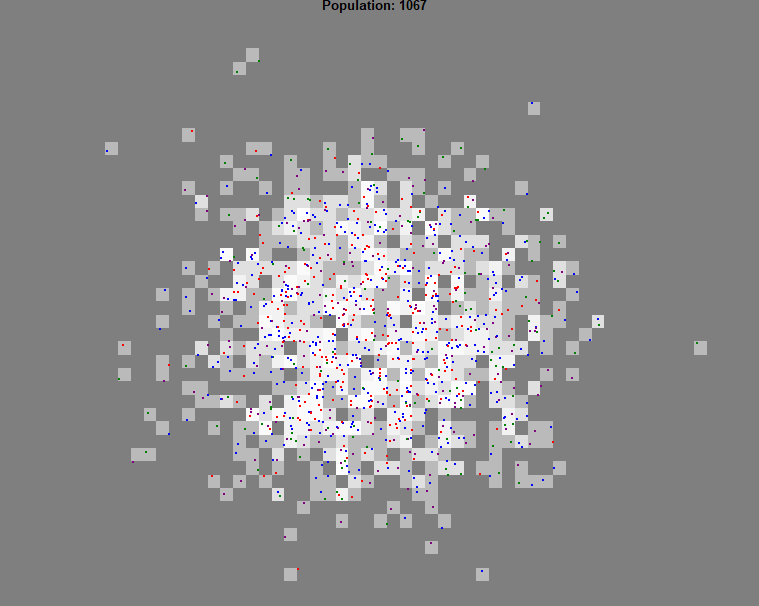
\includegraphics[scale = 0.8]{Graphics/city sim basic.png}
    \caption{Simulation of distribution of city consisting of household with basic psuedo-continuous utilities. Red, blue, purple, and green units represent income levels from lowest to highest respectively.\textsuperscript{\cite{pjcode}}}
    \label{fig:city sim}
\end{figure}